%Lab4
\section{Circuit description}
\label{sec:analysis}

\begin{figure}[h] \centering
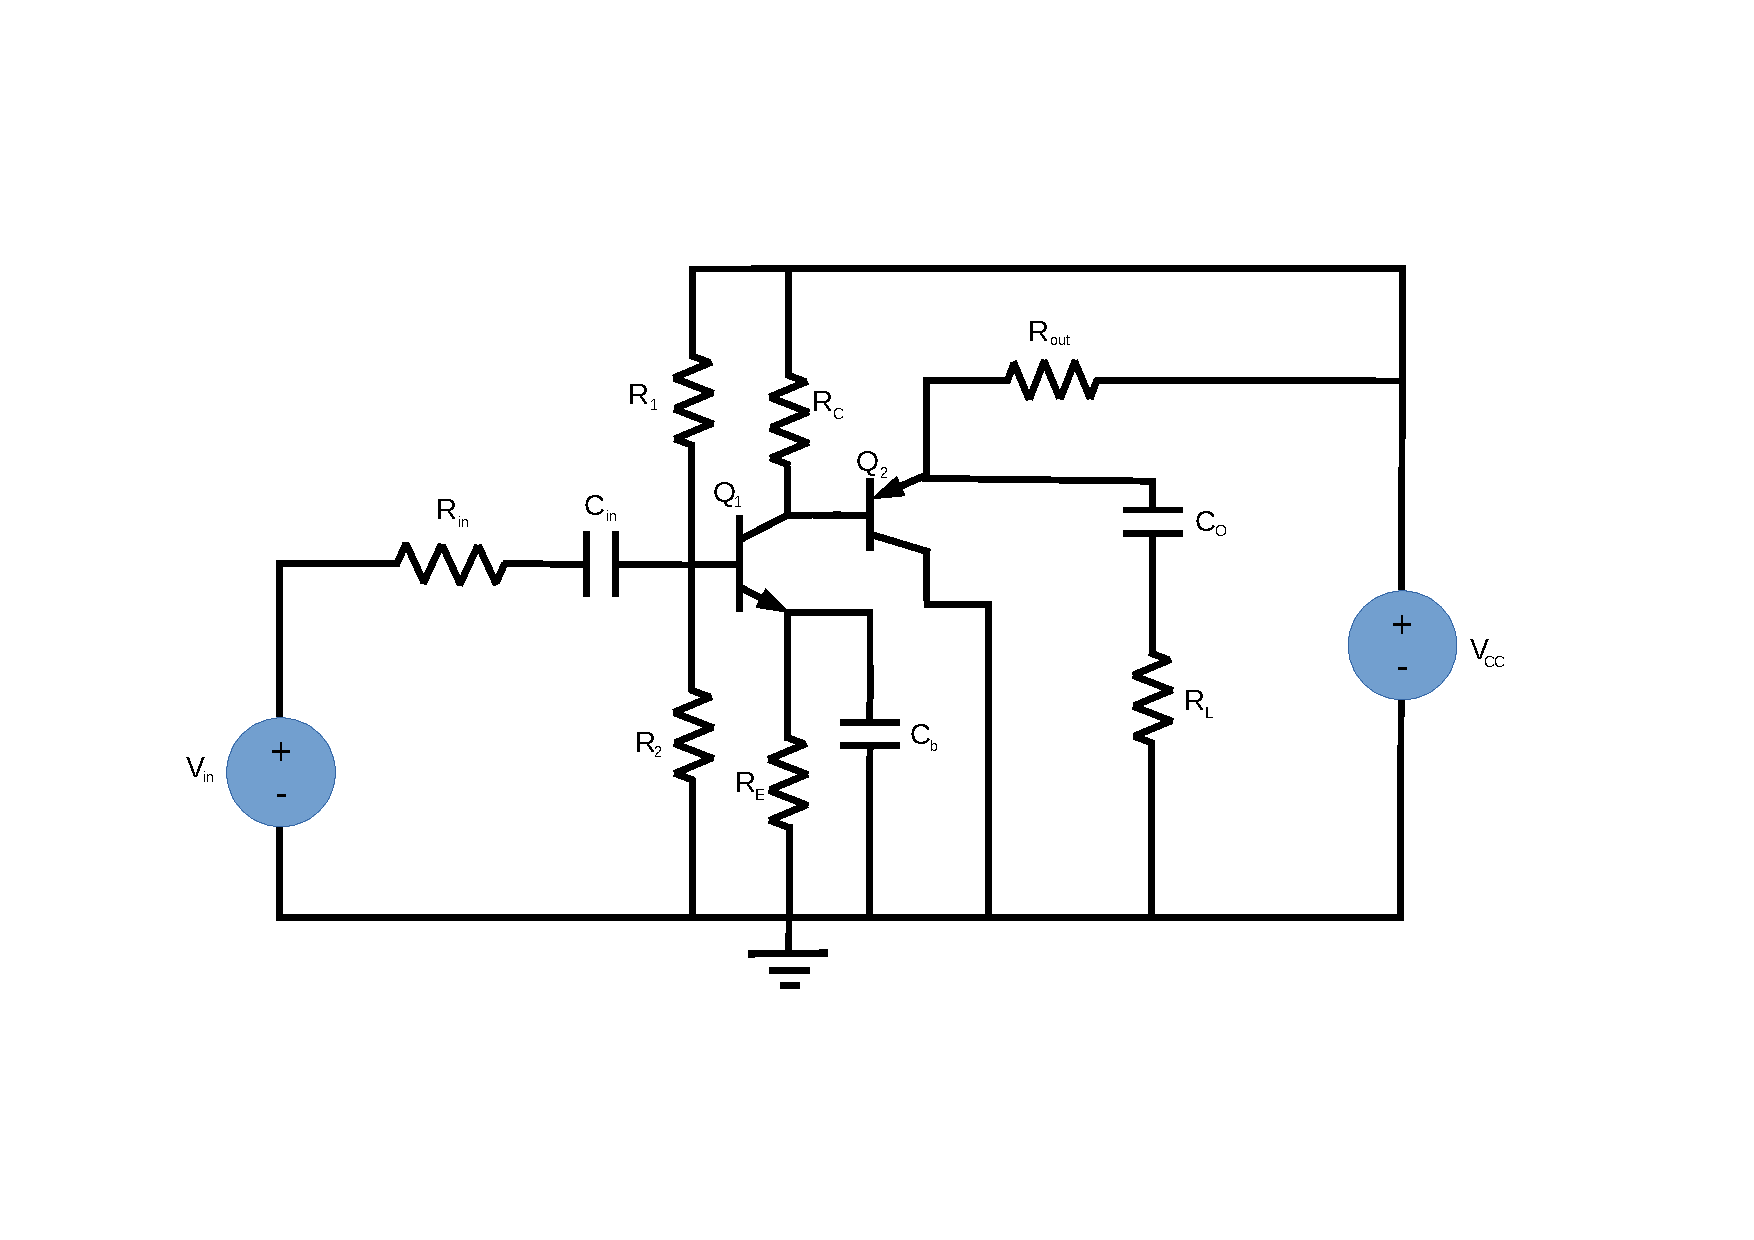
\includegraphics[width=0.9\linewidth]{../figlib/lab4.pdf}
\caption{Circuit to be analysed in this report.}
\label{fig:lab4}
\end{figure}


In the current section, we will describe the circuit shown in Figure \ref{fig:lab4}. 
So in this circuit you can see our final configuration to build an audio amplifier circuit. It is composed by 2 input voltage sources ($V_{in}; V_{CC}$), 
6 resistors ($R_{in}; R_{1}; R_{2}; R_{C}; R_{E}; R_{out}$), 
3 capacitors ($C_{in}; C_{b}; C_{O}$), 2 transistors ($Q_{1}; Q_{2}$),respectively NPN and PNP and a output device (speaker) with a 8 $\Omega$ resistance.
In the table \ref{tab:circuit_values} it can be seen all the components and their respective values.

%verificar a especificação do circuito
%apresentar tabela com os componentes e os seus respetivos valores 

\begin{table}[h]
  \centering
  \begin{tabular}{|l|r|}
    \hline    
    {\bf Name} & {\bf Value [{$\Omega$} or V or F]} \\ \hline
    \input{../mat/Values.tex}
  \end{tabular}
  \caption{Values of the various components and parameters.}
  \label{tab:circuit_values}
\end{table}


\newpage
\section{Circuit Analysis}
\label{sec:circuit}
\subsection{Theoretical analysis}
\label{sub:t1}

In this section, the circuit shown above is analysed theoretically using octave to make the calculations.

To start with, to ensure that the circuit works properly we must see if both transistors are working in forward active region (FAR). In order to achieve that, we started by 
computing the operational point, using the theoretical DC model. To verify the FAR, we must make sure that in NPN transistor $V_{ce}$ (voltage drop between collector and emitter)
must be greater than $V_{be}$ (voltage drop between base and emitter) and in PNP transistor Vec (voltage drop between emitter and collector) must be greater than Veb (voltage
drop between emitter and base).  
The results obtained are shown in the table bellow:

\begin{table}[h]
  \centering
  \begin{tabular}{|l|r|}
    \hline    
    {\bf Name} & {\bf Value [V]} \\ \hline
    \input{../mat/OP.tex}
  \end{tabular}
  \caption{FAR confirmation}
  \label{tab:OP_Values}
\end{table}

As we can see, both differences are positive so we confirm that transistors are working in forward active region.

Then, we analyse some important aspects about the circuit such as impedances and gains. We divide the circuit in its two stages, common emitter and output stage, in order 
to compute their individual properties, after that to obtain the total gain and impedances we analyse the whole circuit.   
Now presenting the tables that allowed us to make some conclusions about these aspects.

\begin{table}[h]
  \centering
  \begin{tabular}{|l|r|}
    \hline    
    {\bf Name} & {\bf Value [{$\Omega$} or dB]} \\ \hline
    \input{../mat/Stage1.tex}
  \end{tabular}
  \caption{Common emitter properties}
  \label{tab:1_Values}
\end{table}

\begin{table}[h]
  \centering
  \begin{tabular}{|l|r|}
    \hline    
    {\bf Name} & {\bf Value [{$\Omega$} or dB]} \\ \hline
    \input{../mat/Stage2.tex}
  \end{tabular}
  \caption{Output stage properties}
  \label{tab:2_Values}
\end{table}

\begin{table}[h]
  \centering
  \begin{tabular}{|l|r|}
    \hline    
    {\bf Name} & {\bf Value [{$\Omega$} or dB]} \\ \hline
    \input{../mat/Final.tex}
  \end{tabular}
  \caption{Total circuit properties}
  \label{tab:T_Values}
\end{table}


In the table \ref{tab:1_Values} we have the common emitter properties and according to the values we can say that the gain and the input impedance achieve the wanted high
values, but the output impedance is too high and because of that we would have degradation of the signal due to low load resistance. To fix this problem we introduce an 
output stage whose properties are shown in table \ref{tab:2_Values}, where we have much lower output impedance and almost an unitary gain, meaning that we won't have 
significant signal loss. When connected together the final circuit won't keep the output stage impedance neither the gain will be the simple multiplication of both gains,
because the circuits interact with each other and the output impedances will be slightly different as the gains (Gainapprox is simple multiplication and Gain is the one
obtained building incremental total circuit).
Since the differences are small and the final gain is similar to stage one gain we can conclude that they can be connected without a significant signal loss.

To close up the theoretical analysis we compute the frequency response of the circuit. Due to the presence of coupling capacitors we considered that the frequency displayed
in $x$ axis corresponds to the frequencies where the capacitor is operating in the bypass region thus the gain being constant.    


\begin{figure}[h] \centering
\includegraphics[width=0.60\linewidth]{gaint.eps}
\caption{Gain in frequency}
\label{fig:1}
\end{figure}


\subsection{Simulation analysis}
\label{sub:s1}


In this section, the circuit shown above is simulated with ngspice.

Same as in the theoretical analyses we started by ensuring that both the transistors were working on the forward active region, to achieve this we simulated the operational
point and made the calculations for the voltages $V_{ce}$, $V_{be}$, $V_{ec}$ and $V_{eb}$, the same as the ones described before.

\begin{table}[h]
  \centering
  \begin{tabular}{|l|r|}
    \hline    
    {\bf Name} & {\bf Value [V]} \\ \hline
    \input{../mat/tableop_tab.tex}
  \end{tabular}
  \caption{FAR confirmation}
  \label{tab:OP1_Values}
\end{table} 

Once again we can see that both transistors are operating in FAR. 

Now we present the measurements for the output voltage gain, both lower and upper cut off frequencies, bandwidth and input/output impedances. 

\begin{figure}[h] \centering
\includegraphics[width=0.5\linewidth]{gaintf.pdf}
\caption{Gain in frequency}
\label{fig:2}
\end{figure}

To measure the output voltage gain we divide the voltage in load by the input voltage obtaining the graph \ref{fig:2}.



To measure the values in table \ref{tab:low_Values} we found the maximum value of output voltage and determined the frequencies where the output voltage was 3 dB lower than 
the maximum value. The bandwidth was calculated as the difference of cut off frequencies.

\begin{table}[h]
  \centering
  \begin{tabular}{|l|r|}
    \hline    
    {\bf Name} & {\bf Value [Hz]} \\ \hline
    \input{../mat/tableband_tab.tex}
  \end{tabular}
  \caption{Bandwidth and cut off frequencies}
  \label{tab:low_Values}
\end{table} 

\begin{figure}[h!]
            \centering
            \subfigure[]{\includegraphics[width=0.45\textwidth]{in_imp.pdf}} 
            \subfigure[]{\includegraphics[width=0.45\textwidth]{out_imp.pdf}} 
            \caption{a) Input impedance in frequency b) Output impedance in frequency}
            \label{fig:3}
\end{figure}


In the figure \ref{fig:3} we can see the output and input impedances measured for the circuit. To calculate the input impedance we measured the current across the voltage 
source and the voltage drop between the voltage source and the resistor, $R_{in}$, and finally we made the ratio between that voltage and the current. On the other hand for
the output impedance we shut down the input voltage source and we replaced the resistor $R_{L}$ by an ac voltage source, so that when we made the ratio between the voltage in 
this voltage source and the current flowing through it we will get the output impedance.     

\newpage

In both stages there are some important components which give the circuit a better behaviour. To start with the coupling capacitors, there is one in the input and one in
the output and they allow us to achieve higher length in the bandwidth because they block the Dc component of the input voltage (behaves like an open circuit to low
frequencies). 

Other important component is the bypass capacitor. It brings to the output a much more stable bandwidth this meaning a wider range of frequencies where the gain is almost 
maximum, because it will behave like an open circuit to low frequencies and a short circuit to high frequencies. 

The last component that we are talking about is the resistor $R_{C}$. The incremental analysis shows that the final gain depends proporcionally of $R_{C}$ so if we 
increase $R_{C}$, the gain also increases.


\subsection{Comparation of results} %isto e para mudar so precisava do label
\label{sub:comp}

In this subsection, we will compare the results of the two previous subsections, more concretely, we will compare the gain, the impedances and the OP results.
Starting with the OP results we already confirm that both are working in FAR but the results are a little different between them as we can see from tables \ref{tab:OP_Values}
and \ref{tab:OP1_Values}, because in theoretical results we assume the maximum voltage drop possible in $V_{be}$ and $V_{eb}$ so the ($V_{ce}$-$V_{be}$) and ($V_{ec}$-$V_{be}$) is 
lower in theoretical results.

Now looking to the impedances of all circuit, they are close to each other but they aren't equal because in theoretical analysis we consider that capacitors behave like 
short circuits and ngspice doesn't do that (it uses more complex methods to obtain impedances).

To finish we compare the final gain of both analysis, we can observe from graphs \ref{fig:1} and \ref{fig:2} that theoretical analysis has an higher gain than ngspice's 
and that's because there might be some voltage depletion in the capacitors that is taken in account in ngspice's analysis.

\newpage
\section{Discussion of results}
\label {sec:aspects}

The objetive was improving an audio amplifier and achieve the best merit. The merit is given by equation \ref{eq:1} and the decisions were made in order to increase the 
numerator (gain and bandwidth) of the equation and decrease the denominator (cost and lower cut off frequency).
\begin{equation}
M=\frac{voltageGain*bandwidth}{cost*lowercutoffFrequency}
\label{eq:1}
\end{equation}

Before discussing our final results we would like to explain some of the decisions as well as explore the impact of changing of values of some specific components.
Two of the most important components that we change are the coupling capacitors. As we already explained we need to have them to increase the bandwidth and if we increase 
them we would have a better bandwitdh and a lower cut off frequency, but to do that we need to spend more money. So we tried to find the best ratio of those quantities.
We also noticed that output capacitor needed to be greater than input capacitor to achieve better results. 

The same idea was used in the value for the bypass capacitor, since when we increased its capacitance we are stabilizing the bandwidth as well as increasing its length,
being its final value a cumulative of incremental experiences. 

Lastely, we explore the influence of the resistance related with $R_{C}$ and, purely by experience we realized that when increasing its value the gain would increase, but
the length of the bandwidth would decrease and vice-versa, so we had to find incrementaly the best result we could achieve.

As for our final circuit, the results we obtained to the various properties taken in account in the merit formula were the following:

\begin{table}[h]
  \centering
  \begin{tabular}{|l|r|}
    \hline    
    {\bf Name} & {\bf Value [Hz]} \\ \hline
    \input{../mat/tablefinal_tab.tex}
  \end{tabular}
  \caption{Circuit final results}
  \label{tab:merit}
\end{table} 

Looking to the table we can see that we achieved a very good bandwidth (we can work in all audible frequencies by humans) and an high gain will keeping the circuit cost 
relatively low resulting in an acceptable merit. 
